\documentclass{article}
\usepackage{epsfig, latexsym}

\begin{document}

\newcommand{\SOPmin}{${\rm SOP}_{\rm min} \ $}
\newcommand{\POSmin}{${\rm POS}_{\rm min} \ $}
\newcommand{\bs}{\backslash}


\title{
\Huge{CSE 271 -- Spring 2004}\\
\normalsize{Exam 2}\\
\makebox[4in][l]{Name:}
SSN:}
\date{}

\maketitle{}

\begin{tabular}{llll}
\begin{tabular}{c||c}
D & Q+   \\ \hline
0 & 0 \\ \hline
1 & 1 \\
\end{tabular}
&
\begin{tabular}{c||c}
T & Q+   \\ \hline
0 & Q \\ \hline
1 & Q' \\
\end{tabular}
&
\begin{tabular}{c|c||c}
S & R & Q+   \\ \hline
0 & 0 & Q \\ \hline
0 & 1 & 0 \\ \hline
1 & 0 & 1 \\ \hline
1 & 1 & x \\
\end{tabular}
&
\begin{tabular}{c|c||c}
J & K & Q+   \\ \hline
0 & 0 & Q \\ \hline
0 & 1 & 0 \\ \hline
1 & 0 & 1 \\ \hline
1 & 1 & Q' \\
\end{tabular}
\\
\end{tabular}


\begin{enumerate}

\item {\bf (1 pt.)} Assuming a word size of 5 bits, interpret 11010 as a 2's complement
number.
\begin{description}
\item{a) }-24
\item{b) }-2
\item{c) }-12
\item{d) }-6
\item{e) }None of the above.
\end{description}

\item {\bf (1 pt.)} Assuming a word size of 4 bits, determine the 2's complement
representation of -5.
\begin{description}
\item{a) }1011
\item{b) }1101
\item{c) }1011
\item{d) }1001
\item{e) }None of the above.
\end{description}

\item {\bf (1 pt.)}How many 3:8 decoders does it take to build a 4:16 decoder?
\begin{description}
\item{a) }2
\item{b) }3
\item{c) }4
\item{d) }16
\item{e) }Trick question, you cannot build a 4:16 decoder with 3:8 decoders.
\end{description}


\item {\bf (1 pt.)} If the delay through a single 2:1 mux is 1 unit of time then
what is the propagation delay through a 16:1 mux constructed from 2:1 muxes?
\begin{description}
\item{a) }2
\item{b) }4
\item{c) }8
\item{d) }15
\item{e) }None of the above.
\end{description}

\item {\bf (1 pt.)} How many inputs do the AND gates in a 8:1 mux have?
\begin{description}
\item{a) }2
\item{b) }4
\item{c) }8
\item{d) }16
\item{e) }None of the above.
\end{description}

\item {\bf (1 pt.)} How many 2:1 muxes are needed to construct a 8x4x1 mux?
\begin{description}
\item{a) } 4
\item{b) } 8
\item{c) } 12
\item{d) } 18
\item{e) } 24
\end{description}

\item {\bf (2 pt.)} Which of $G,L,E$ below must be connected to the
sel input of the mux so that \\
\verb+if (X >=  Y) then Z = X else Z = Y;+

%% 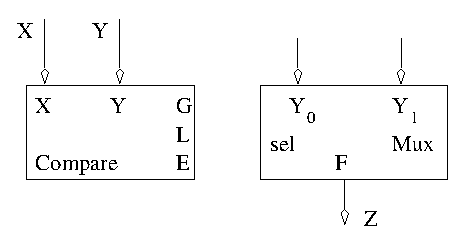
\includegraphics{./Fig2/compare2}

\begin{description}
\item{a) } G
\item{b) } L
\item{c) } E
\end{description}

\pagebreak
\item {\bf (2 pt.)} Consult the figure associated with question
7.  Which of $X,Y$ must be connected to the
$y_0$ input of the mux so that \\
\verb+if (X >=  Y) then Z = X else Z = Y;+

\begin{description}
\item{a) } X
\item{b) } Y
\end{description}

Questions 9-11 concern the following 16x1 mux constructed from 4x1 muxes.  
Note the odd arrangement of the select lines and the order of the y inputs.
%% \includegraphics[-60mm,125mm][0mm,51mm]{./Fig2/OddMux}


\item {\bf (1 pt.)} What input corresponds to $A$?
\begin{description}
\item{a) } $y_{11}$
\item{b) } $y_{12}$
\item{c) } $y_{13}$
\item{d) } $y_{14}$
\item{e) } none of the above.
\end{description}

\item {\bf (1 pt.)} What input corresponds to $B$?
\begin{description}
\item{a) } $y_5$
\item{b) } $y_6$
\item{c) } $y_7$
\item{d) } $y_8$
\item{e) } none of the above.
\end{description}

\item {\bf (1 pt.)} What input corresponds to $C$?
\begin{description}
\item{a) } $y_0$
\item{b) } $y_1$
\item{c) } $y_2$
\item{d) } $y_3$
\item{e) } none of the above.
\end{description}

\pagebreak
\underline{For questions 12-15 use the circuit and timing diagram
show below}

%% \scalebox{0.7}{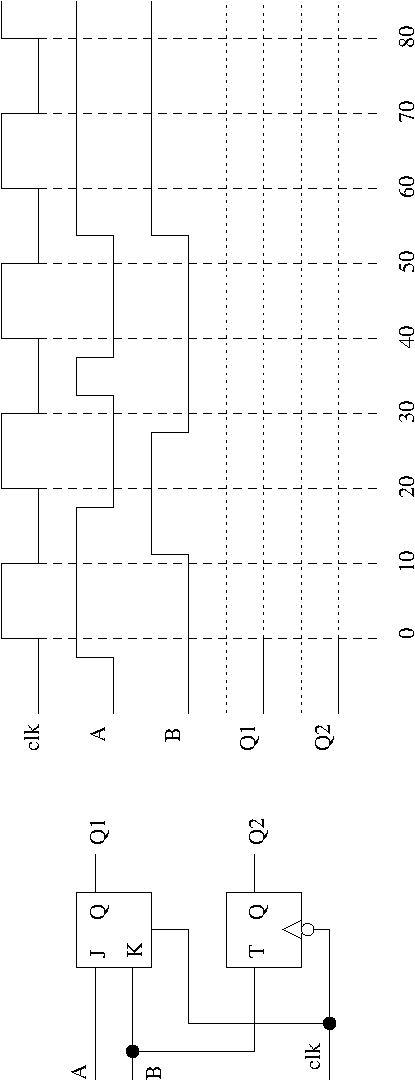
\includegraphics{./Fig2/ExTim3}}

\item {\bf (1 pt.)} What is the value of $Q_1$ at time=25nS?
\begin{description}
\item{a) }0 
\item{b) }1 
\item{c) }Toggling rapidly. 
\item{d) }Input(s) is (was) changed too close to the clock edge to tell.
\end{description}

\item {\bf (1 pt.)} What is the value of $Q_1$ at time=65nS?
\begin{description}
\item{a) }0 
\item{b) }1 
\item{c) }Toggling rapidly. 
\item{d) }Input(s) is (was) changed too close to the clock edge to tell.
\end{description}

\item {\bf (1 pt.)} What is the value of $Q_2$ at time=25nS?
\begin{description}
\item{a) }0 
\item{b) }1 
\item{c) }Toggling rapidly. 
\item{d) }Input(s) is (was) changed too close to the clock edge to tell.
\end{description}

\item {\bf (1 pt.)} What is the value of $Q_2$ at time=55nS?
\begin{description}
\item{a) }0 
\item{b) }1 
\item{c) }Toggling rapidly. 
\item{d) }Input(s) is (was) changed too close to the clock edge to tell.
\end{description}

\pagebreak
For questions 16,17 assume that a 4-bit (arithmetic) shift register 
has the following truth table.   Complete the timing diagram below.

\begin{tabular}{l|l|l||l}
clk             & $C_1 C_0$     & D & $Q^+$     \\ \hline
0,1,$\downarrow$& xx            & x & Q         \\ \hline
$\uparrow$      & 00            & x & Q         \\  \hline
$\uparrow$      & 01            & x & $q_3$\&$Q>>1$ \\  \hline
$\uparrow$      & 10            & x & $Q<<1$\&0 \\  \hline
$\uparrow$      & 11            & D & D         \\
\end{tabular}

%% \scalebox{0.7}{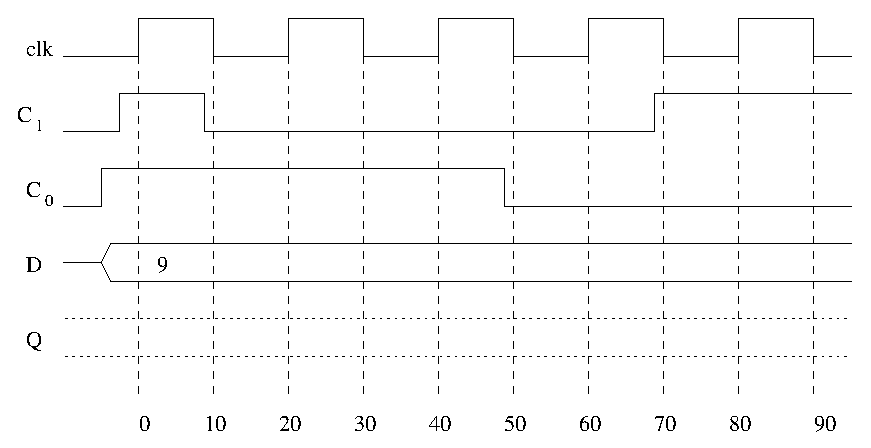
\includegraphics{./Fig2/shift-time2.eps}}

\item {\bf (2 pt.)}What is the value of $Q$ at time 55?

\begin{tabular}{p{0.6in} p{0.6in} p{0.6in} p{0.6in} l}
a) 0001 & b) 0010 & c) 0100 & d) 1110 & e) none of the above
\end{tabular}

\item {\bf (2 pt.)}What is the value of $Q$ at time 90?

\begin{tabular}{p{0.6in} p{0.6in} p{0.6in} p{0.6in} l}
a) 0001 & b) 0010 & c) 0100 & d) 1110 & e) none of the above
\end{tabular}

For questions 18,19 use the following truth table for a 4-bit
counter. Use the values from the timing diagram as inputs
to the counter and answer the questions below.

\begin{tabular}{l|l|l||l}
clk             & $C_1 C_0$     & D & $Q^+$     \\ \hline
0,1,$\downarrow$& xx            & x & Q         \\ \hline
$\uparrow$      & 00            & x & Q         \\  \hline
$\uparrow$      & 01            & x & Q+1 mod 16\\  \hline
$\uparrow$      & 10            & x & Q-1 mod 16\\  \hline
$\uparrow$      & 11            & D & D         \\
\end{tabular}

\item {\bf (2 pt.)}What is the value of $Q$ at time 35?

\begin{tabular}{p{0.6in} p{0.6in} p{0.6in} p{0.6in} l}
a) 1000 & b) 1001 & c) 1010 & d) 1011 & e) none of the above
\end{tabular}

\item {\bf (2 pt.)}What is the value of $Q$ at time 75?

\begin{tabular}{p{0.6in} p{0.6in} p{0.6in} p{0.6in} l}
a) 1000 & b) 1001 & c) 1010 & d) 1011 & e) none of the above
\end{tabular}


\pagebreak
For problems 20-24 use the following figure and timing diagram.
You should assume that all the devices process 5-bits data 
values.

%% 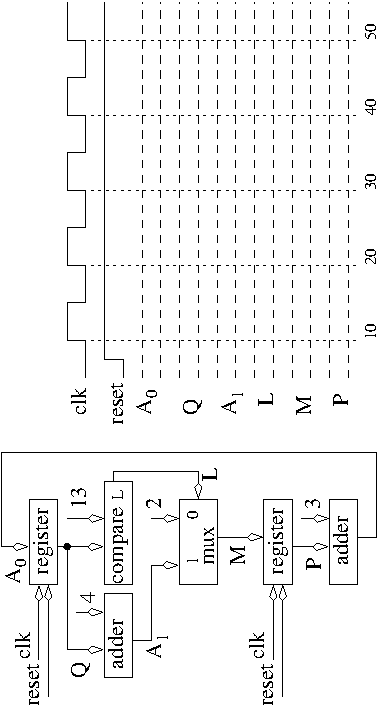
\includegraphics{./Fig2/BBBtiming3}

\item {\bf (2 pt.)}What is the value of $P$ at time 15?

\begin{tabular}{p{0.6in} p{0.6in} p{0.6in} p{0.6in} l}
a) 0  & b) 3  & c) 4  & d) 6  & e)  11
\end{tabular}

\item {\bf (2 pt.)}What is the value of $A_0$ at time 25?

\begin{tabular}{p{0.6in} p{0.6in} p{0.6in} p{0.6in} l}
a) 3  & b) 5  & c) 7  & d) 8 & e) 10
\end{tabular}

\item {\bf (2 pt.)}What is the value of $A_1$ at time 35?

\begin{tabular}{p{0.6in} p{0.6in} p{0.6in} p{0.6in} l}
a) 8  & b) 11  & c) 14 & d) 15  & e) 18
\end{tabular}

\item {\bf (2 pt.)}What is the value of $Q$ at time 45?

\begin{tabular}{p{0.6in} p{0.6in} p{0.6in} p{0.6in} l}
a) 5  & b) 7  & c) 11 & d) 13  & e) 14
\end{tabular}

\item {\bf (2 pt.)}What is the value of $M$ at time 55?

\begin{tabular}{p{0.6in} p{0.6in} p{0.6in} p{0.6in} l}
a) 2  & b) 5  & c) 7 & d) 8  & e) 9
\end{tabular}

\pagebreak
\item {\bf (4 pt.)}Describe the sequence of bits seen on the
$Q$ output.  Write down the output sequence until it starts to
repeat, write down the first repeated value.  Assume that 
$Q=0100$ initially.

\begin{tabular}{l|l|l|l||l|r}
clk         & $C_1 C_0$ & D & cin & $Q^+$ & comment \\ \hline \hline
0,1,$\downarrow$ & xx   & x & x   & Q     & hold     \\ \hline
$\uparrow$     & 00     & x & x   & Q     & hold     \\  \hline
$\uparrow$     & 01     & x & cin & $cin,Q_3,Q_2,Q_1$  & shift right \\  \hline
$\uparrow$     & 10     & x & cin & $Q_2,Q_1,Q_0,cin$  & shift left \\  \hline
$\uparrow$     & 11     & D & x   & D     & parallel load  \\
\end{tabular}

%% \psfig{figure=./Fig2/shift.eps,height=1.5in.}

\end{enumerate}
\end{document}
